\documentclass[11pt,english]{article}

% Set page margins correctly
\usepackage{geometry}
\usepackage{url}
\geometry{letterpaper,top=1.0in,left=1.0in,bottom=1.0in,top=1.0in,headsep=6pt,footskip=18pt}

\usepackage{lscape}
\usepackage[square,comma,numbers,sort&compress]{natbib}

% Use fancy header style
\usepackage{fancyhdr}
\pagestyle{empty}
\renewcommand{\headrulewidth}{0.75pt}
\renewcommand{\footrulewidth}{0.75pt}
\usepackage{setspace}
\usepackage{listings}
\usepackage{float}
\floatstyle{plain}
\newfloat{command}{thp}{lop}
\floatname{command}{Command}
\doublespacing
\usepackage{boxedminipage}
\usepackage{graphicx}
\usepackage{amsmath,amsfonts}
\usepackage{babel,verbatim}
\usepackage{enumerate}
\usepackage{longtable}
\usepackage{multirow}
\usepackage{sectsty}
\usepackage[compact]{titlesec}
\usepackage[usenames]{color}
\usepackage{ulem}
\usepackage{multirow,booktabs,ctable,array}
\graphicspath{{./Figures/}
                          }

%\DeclareMathOperator*{\argmax}{arg\,max}
\newcommand{\argmax}{\operatornamewithlimits{argmax}}
\newcommand{\argmin}{\operatornamewithlimits{argmin}}

\long\def\symbolfootnote[#1]#2{\begingroup%
\def\thefootnote{\fnsymbol{footnote}}\footnote[#1]{#2}\endgroup}

    \usepackage{color}

    \definecolor{listcomment}{rgb}{0.0,0.5,0.0}
    \definecolor{listkeyword}{rgb}{0.0,0.0,0.5}
    \definecolor{listnumbers}{gray}{0.65}
    \definecolor{listlightgray}{gray}{0.955}
    \definecolor{listwhite}{gray}{1.0}

\begin{document}
\normalem

\vspace*{5cm}

\begin{center}
{\Large \bf Multivariate EM Segmentation Project} \\
\vspace*{0.5cm}
{\normalsize Ben Kandel, Pengfei Zheng and Brian B. Avants$^1$} \\
\begin{singlespace} 
{\scriptsize  $^1$ Penn Image Computing and Science Laboratory, University of Pennsylvania, Philadelphia, Pennsylvania,  USA.}
\end{singlespace}
\end{center}

\vfill

\begin{singlespace} 
\scriptsize
\flushleft
%\line(1, 0){250} \\
{\bf MVSeg}\\
Corresponding author: \\
Brian B. Avants\\
3600 Market Street, Suite 370\\
Philadelphia, PA  19104\\
avants@picsl.upenn.edu\\
\end{singlespace} 
\clearpage
\begin{abstract} 
Neuroanatomical coordinate systems are essential for the
interpretation of structural and functional imaging studies.  However,
manual delineation of the neuroanatomical complex is time consuming
and prone to random performance variability.  This work describes an
open source, image-based approach to white matter parcellation which
uses training data to propagate structural labelings to individual
images.  The Bayesian formulation of the segmentation problem is
solved using the Expectation Maximization (EM) algorithm with a
variety of different multivariate distance metrics.  We evaluate our
ability to segment DTI data based on comparison with
registration-based approaches and biological validity of results.
\end{abstract}

\section{Introduction}
The Expectation-Maximization (EM) framework \citep{Dempster1977} is a
powerful optimization method for parameter estimation.  This project
will investigate EM with application to diffusion tensor imaging and
will test our ability to segment major white matter tracts in
different subjects.   

\section{Data}
\subsection{DTI}
We can start small with a couple of interesting datasets. 

\noindent $I$ High-resolution human DT atlas in nifti format: \url{http://www.nitrc.org/frs/?group_id=432}

\noindent $J$ A second human DT atlas
\url{http://www.nitrc.org/projects/dtitk} which also has labels that
may be used to guide our parcellation of the white matter into major
tracts.

\noindent $K$ A similar atlas for macaque \url{http://www.nitrc.org/projects/rmdtitemplate}

Segmenting these templates into similar regions will let us quantify
differences in white matter due to aging in humans ($I$ vs $J$) and
between humans and macaques ($I$ and $J$ vs $K$).

Once we establish a working knowledge of DTI segmentation, we can
evaluate reproducibility of our methods on the Kirby dataset
\url{http://www.nitrc.org/projects/multimodal/}.  This unique
collection of images has repeat imaging on the same subject within a
week.  Thus, our segmentation tools should provide repeatable
measurements of volume or tracts across all subjects.  Once
repeatability is established, we can apply the segmentation approach
to other datasets where investigating population differences is of
interest.

\begin{figure}
\begin{center}
\begin{tabular}{c}
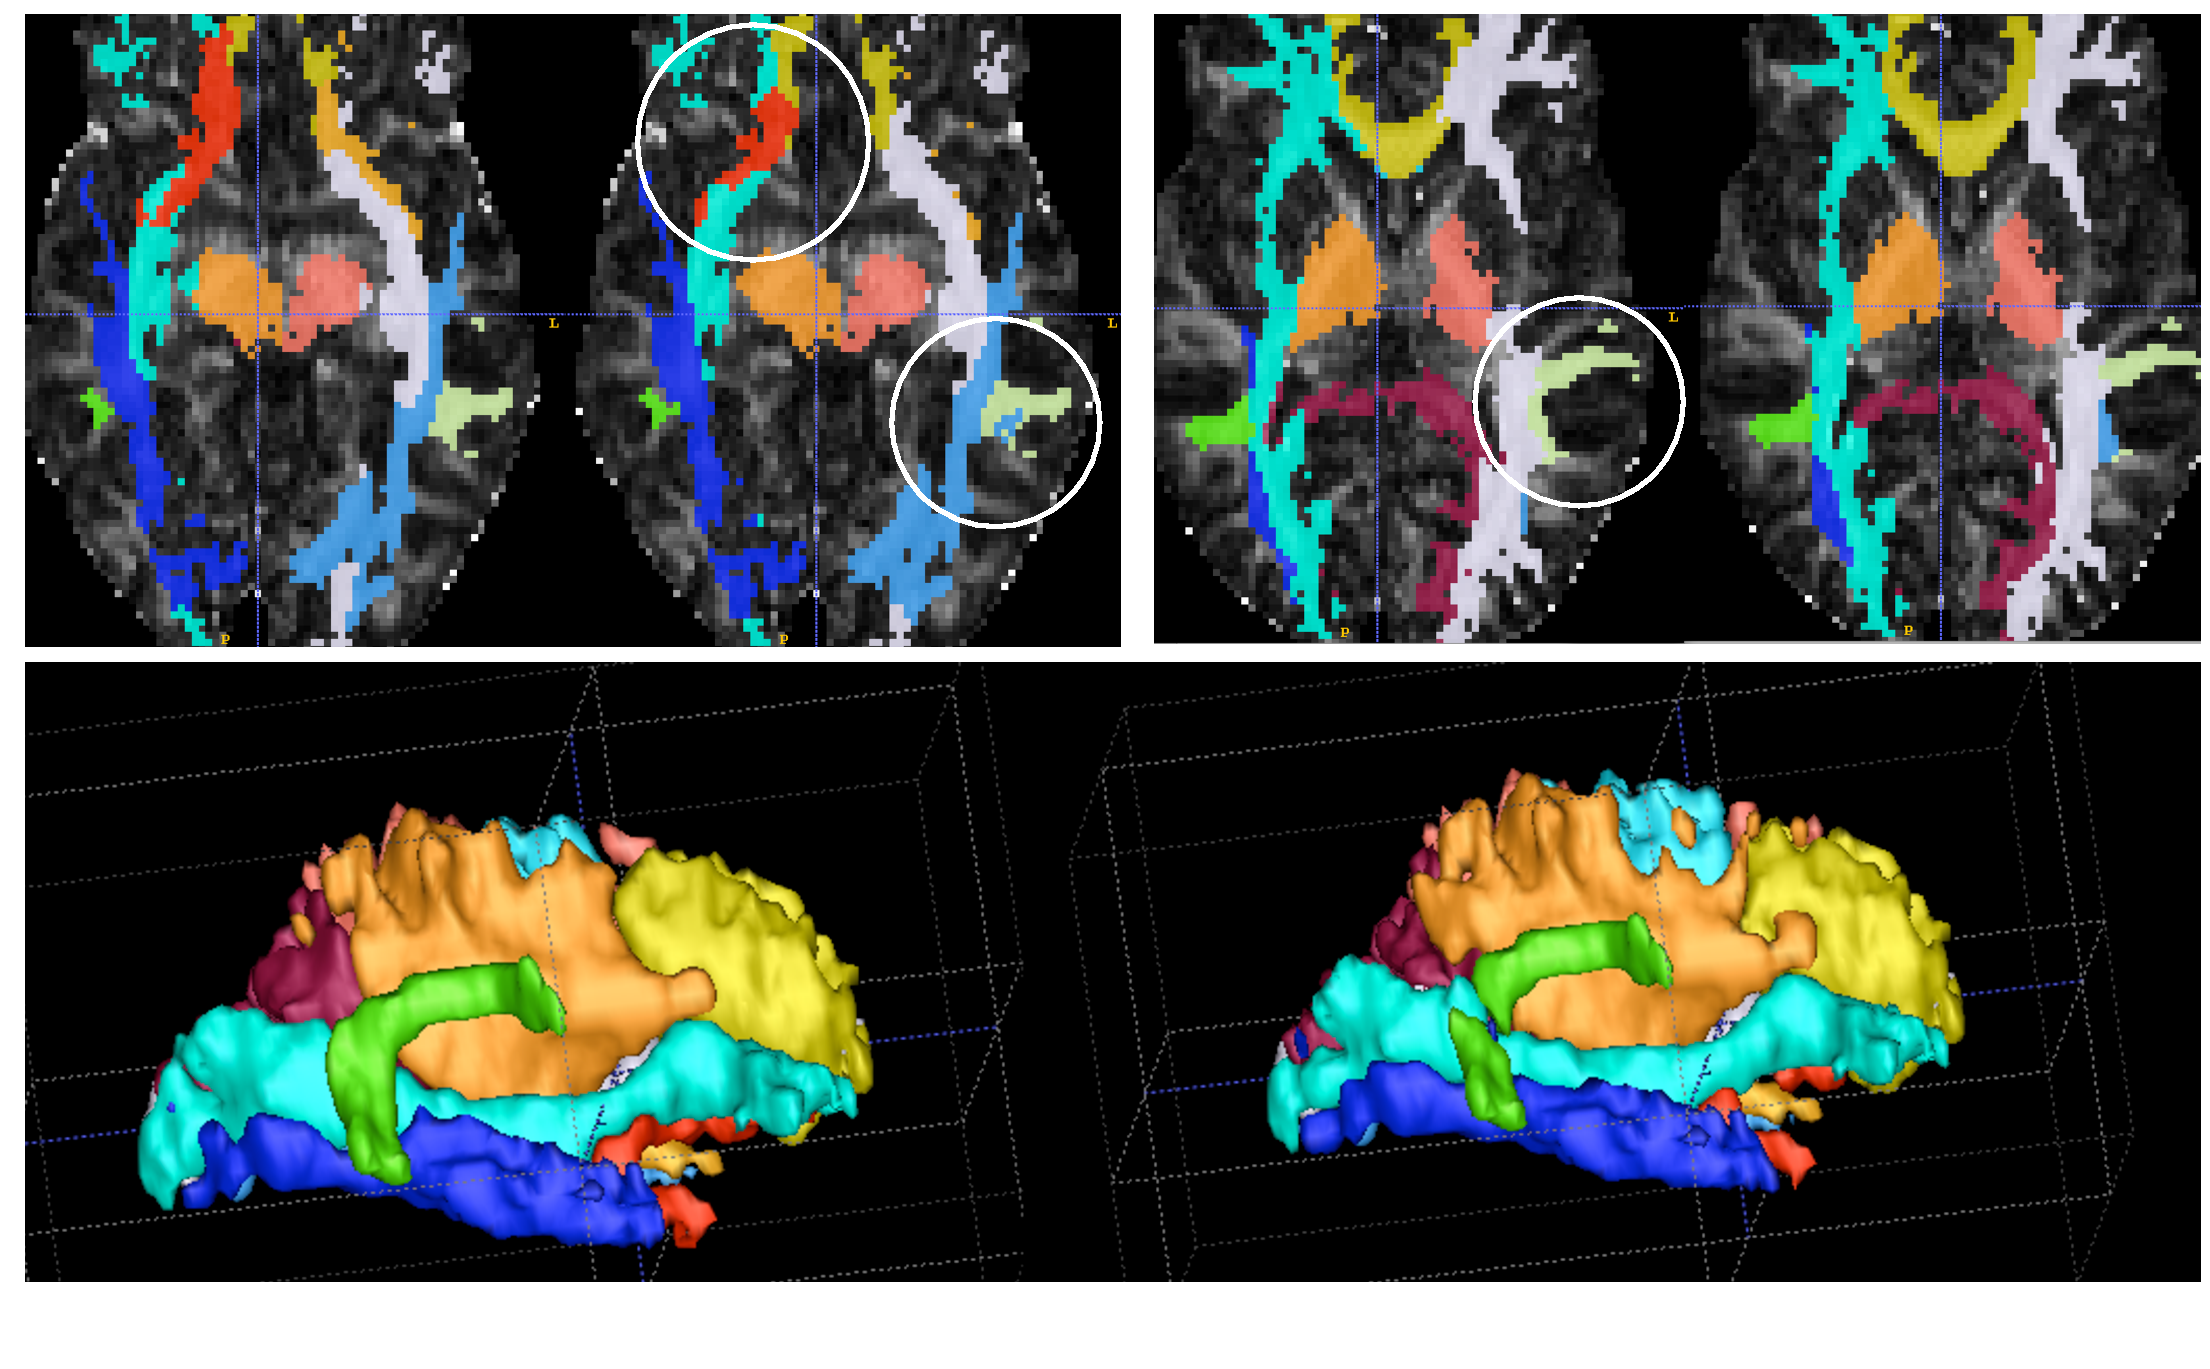
\includegraphics[width=6in]{Figures/004_vec_vs_dti.pdf}
\end{tabular}
\caption{The tensor-based segmentation on the left and the
  RGB vector segmentation is on the right.  Both use Mahalanobis
  distance and EM optimization with spatial priors.}
\label{fig:example1}
\end{center}
\end{figure}

\subsection{Neonate T1 and T2} There is also an interesting neonatal
dataset for which there is some multivariate data (T1 and T2).  The
goal with the neonatal segmentation is to increase repeatability
between automated and manual volume measurements.  We do fairly well
already but could improve results with some additional work on, for
instance, distance metrics and/or partial volume estimation.

\section{Methods} Our goal will be to provide reproducible
measurements derived from multivariate segmentation.
\begin{description}
\item[RBG:] The principal direction of the tensor can be visualized in
  RGB space.  Some segmentation methods rely on this feature 
  modulated by the FA.
\item[FA:] Fractional anisotropy derived from the tensor.  This is
  equal to the variance of the eigenvalues of the tensor matrix.  It
  is the most common measure used in DTI studies, along with
  tractography. 
\item[Tractography:] White matter tracts provide a physical connection
  between and within cortical regions.  At the coarse scale of DTI, we mostly
  look at connections between cortical regions.  A simple way to
  define a tract from DTI is to follow the principal eigenvector until
  some stopping criterion based on curvature or FA is reached. 
\end{description}
An EM segmentation method can use any of these features.  One project
that may be similar to our own is here
\url{http://www.nitrc.org/projects/dots} though there is no clear
reference other than the website.  Prior DT segmentation work is here
\citep{Lenglet2005} and here \citep{Awate2007}.  Classic work on
partial volume estimation \citep{Santago1993,Shattuck2001}.


We can also explore the effect of simulated and/or deterministic
annealing which is a hidden feature of Atropos. 

\section{Results}

\section{Discussion}

\paragraph{Information Sharing Statement}
{Atropos software is available in ANTs
    {\color{blue}{\url{http://www.picsl.upenn.edu/ANTs}}}
which depends on ITK {\color{blue}{\url{http://www.itk.org/Wiki/ITK/Git/Download}}}.
BrainWeb provides good evaluation data
{\color{blue}{\url{http://mouldy.bic.mni.mcgill.ca/BrainWeb/}}}.
ITK-SNAP is useful for scalar and RGB visualization {\color{blue}{\url{www.itksnap.org}}}.

\paragraph{Acknowledgments}
{This work was supported in part by NIH (AG17586, AG15116, NS44266, and
NS53488).}

\newpage

\bibliographystyle{plain}
\bibliography{MVSeg} 
\end{document}
